\chapter{Simulation Structure}\label{simulation_structure}
%%%%%%%%
%%%%%%%% Scenario and Simulator
%%%%%%%%
\section{Scenario and Simulator}\label{scenario_and_simulator}

\subsection{Context}

The Platform presents an environment consisting of people subjected to a life within a tower. This tower has a predefined set of laws that closely control the people’s lives, and it is ultimately up to these individuals to act however they suppose is correct.
 
The tower is made up of multiple floors with one agent per floor, starting with Floor 1 at the top and increasing downwards. Above Floor 1, there is a kitchen which produces a fixed amount of food per day.
The floor on which people are based is random, and periodically reshuffles with a fixed frequency. At the beginning of each day a platform begins moving down the tower, starting from the top floor where it is loaded with food and stopping for a constant time at each floor. Over a period of time, there is enough food on the platform to minimally satisfice the agents, but not maximally satisfy them all.
 
The people exist with limited knowledge of tower; they must eat enough within a period to survive and can communicate with other individuals on local floors. They know which floor they are on, but do not know how many floors there are in the tower nor how much food there is at the beginning of each day. Additionally, the people in the tower do not explicitly know how often the reshuffle period is. Finally, when a person dies, they are immediately replaced.

The scenario presented above is heavily influenced by \textit{`El Hoyo'}\citep{elhoyo2019} (translating directly to `The Hole') a Spanish film released in 2019.

\subsection{Assumptions}


There are several assumptions from the given context and, for the implementation in this project, are described in this section.

\begin{enumerate}
    \item  Pre-existing knowledge -- people exist in the tower with a level of knowledge of their environment; this reduces the amount of learning required before action can take place. Pre-existing ideologies are included in this: people have their ways of interacting with others, views on socialising and the like, perhaps acquired from a life before the tower.
     Basic concepts such as consuming food to increase health are known.
      \item  Taking food -- people are allowed to take as much food from the platform as they are able to eat. They cannot preserve food to eat on separate days. Additionally, the utility of the food taken decreases exponentially (each unit of food has a decreasing improvement to HP) -- representing the law of diminishing returns.
      \item An honest environment -- people are assumed to be truthful: direct deceit does not exist. There are very specific conditions in which deceit is permitted, these will be discussed alongside the introduction of the relevant features, but is related to breaking agreements in times of extreme need.

\end{enumerate}

\subsection{Observations \& Understanding}

An initial observation of the context immediately presents the concept of a `world', i.e., the tower, and `agents', i.e.,  the people. These agents interact with one another and the tower, within constraints, and must be able to react and evolve their behaviour to maximise their utility and survival.
 
 
Within the tower there exists a food allocation problem, which is directly related to the survival of agents and forms the core incentive for self-organisation. With a lack of organisation, the tower society would fall victim to the tragedy of the commons -- the common pool resource would deplete, and the overall well-being of society would suffer for the gain of a few individuals. Hence, the crux of this project is a collective action resource management problem, and agents must be equipped with sufficient capabilities and information.
 
The aforementioned capabilities can be split into two sections: those related to the tower and those related to the agent interactions.
 
Within the tower, agent abilities are listed below:
\begin{enumerate}
    \item View Food on Platform -- the agent cannot view the amount of food on the platform unless it is on the agent’s floor or the floor immediately below the agent.
    \item Food Consumption -- agents cannot preserve food. Agents can only eat food from the platform when it is on the agent's floor.
    \item Time Details -- agents do not have explicit access to timed parameters (reshuffle period, day length, time of platform on each floor etc.), however, can use memory to calculate these.
    \item Food Details -- agents do not know the food on the platform at the beginning of each day.

    \item Health Details -- agents do know their current health level and the utility they are receiving from food, as well as how long they can go without food before dying.
    
\end{enumerate}

Agents are also able to communicate with each other:
\begin{enumerate}
    \item Agents should be able to converse with one another and share information.
    \item Agents should be able to form agreements which must be followed.
    \item Agents should be able to differentiate between any new agents that appear locally.
    \item The communication must be limited to single agent interactions and single messages cannot travel past a defined, local distance. 
\end{enumerate}

%%%%%%%%
%%%%%%%%System Design
%%%%%%%%
\section{System Design}\label{system_design}

Based on our initial observations and constraints, possible implementations were explored early on in the design process. Our design process evolved from designing for the simple use case of allowing simple agents to eat food and communicate with primitive messages, to scaling this up to accommodate multiple agents on multiple floors.

\subsection{Ticks and Timing Details}

Discrete time in the simulation is represented by ticks. During each tick, all agents can perform an action such as `eat' or `send a message'. This means that the number of ticks per day restricts the communication between the agents. Moreover, given that messages can only be passed from one floor to one below or above on each tick, we can conclude that certain messages will never get to their receiver. The number of ticks per day is set in the initialisation of the simulation and is the product of the ticks per floor and the number of floors.

\subsection{Agent Configuration}

Agent structures are separated into two different aspects: a base agent and a custom agent, both of which are required to represent a single agent.
The base agent component contains the core information of an agent, including its Health Points, Floor and UUID\footnote{UUID -- Universally Unique Identifier}, as well as a pointer to the tower structure. 
The custom agent contains a pointer to its base agent and any parameters relevant to the specific agent behaviour; this varies between agent types and was implemented by agent teams.

The core parameters of an agent were abstracted out of the custom agent for two reasons:
\begin{enumerate}
    \item Custom agents cannot manipulate their own data or information, rather they can only request access through `getter' functions, which returns either information or an error.
    \item The tower struct has access to the base agents and can therefore influence the agent parameters as determined by the laws existing within the tower. Examples of this include floor reshuffling and health decay.
\end{enumerate}

\subsection{Death and Replacement}

Deaths occur in the tower when an agent has not eaten enough food to stay alive over a certain duration. The nature of replacement in the tower could be of several types:
\begin{enumerate}
    \item Replacing agents with random agent type
    \item Replacing agents with the same agent type
    \item Replacing agents with the dominant agent type
\end{enumerate}

Our design chose to replace agents with the same agent type. While replacing agents with a random agent type would introduce an element of uncertainty, this would have made it difficult to analyse individual agent behaviours. It would have been interesting to experiment with replacing agents with the dominant agent type, however, this posed the question of defining what the most ``dominant'' agent would be.

\subsection{Infrastructure}

Our implementation began with considering the structure of the system given the scenario we had identified. The key required components include a tower that contains agents, with a discrete-time system.
The simulation package holds the state of the tower, base agents, and their corresponding custom agents. The simulation package that creates the world and constructs agents inside a simulation environment. It is the simulation that calls the tower and agent functions to progress the simulation.
The tower is the overall `world' which stores information in its state such as the list of agents, platform level, food available, and tick count. The tower is responsible for updating the platform, reshuffling agents, and replacing dead agents.
The platform is a parameter of the tower and stores the amount of food on the platform and its current floor. It goes down one floor at a predefined tick rate (e.g., every 10 ticks) and it is reset (fill the platform with food and set its floor to 1) at the end of each day.

Base agent contains the core information of an agent, such as an agent's HP and floor. Base agent also contains the \lstinline$hpDecay()$ function as well as a function to calculate an individual agent's utility. 
Custom agents are designed by each of the agent teams, where each one of them has a different strategy.
%%%%%%%%
%%%%%%%% Message Passing
%%%%%%%%
\section{Message Passing}\label{message_passing}
\subsection{Primitive Messaging}
An important role of Team 1 was to design a mechanism for agents to talk amongst each other in the simulation that would allow automated communication. The first step in this process was to design a system which would allow an agent to pass along a minimum viable message to their neighbours. These were the goals of communication in the MVP:
\begin{itemize}
    \item Agents could only talk to their immediate neighbors (+/- 1 floor).
    \item Agents should be given the ability to ignore communication.
    \item Multiple agents could be “speaking” at a given tick.
    \item One agent could send one message per tick.
    \item \textbf{It is entirely an agent's discretion if/when/how they wish to react to a message as long as their behavior is not deceptive}
\end{itemize}
As a team, Team 1 emphasized the last point. The infrastructure should not force any behavior onto the agent as long as the behavior was honest. The basic philosophy of the communication infrastructure was to dictate as little as possible about the agent's behavior while keeping the API friendly, readable and hard to get wrong. This usually meant making providing basic override-able behaviors to be as unobtrusive as possible to team strategies. \newline
The minimum default message had to have the following fields that are accessible to all the agents that receive it:
\begin{itemize}
    \item \textbf{\texttt{MessageType}}: Indicates one of 13 enumerated message types.
    \item \textbf{\texttt{SenderFloor}}: Returns the floor this message was sent from.
    \item \textbf{\texttt{TargetFloor}}: The floor the message is addressed to.
    \item \textbf{\texttt{ID}}: Each message sent is given a unique ID.
\end{itemize}
\vspace{\baselineskip}
For the MVP, Team 1 constructed a system where for example in a scenario where Alice (currently at floor 10) wishes to send a message upward:
\begin{enumerate}
    \item At Tick 0, Alice would construct the message for Bob containing the following information:
        \begin{itemize}
            \item \textbf{Alice's ID}
            \item \textbf{Alice's current floor}: 30
            \item \textbf{Message's target floor}: 31 \textit{Since Alice wants to message the floor above her}
            \item \textbf{Message Type} (to be elaborated on the Common Languages Section)
        \end{itemize}
    \item Still at Tick 0, Alice calls \texttt{SendMessage} which takes her message and passes it to the tower.
    \item The tower acts as the communication authority, finding the agent who is on floor 31 at Tick 0 and inserts the message into the recipient agent's (Bob's) inbox.
    \item At Tick 1, Bob may choose to call \texttt{ReceiveMessage} which would extract Alice's message (if Alice was the first or only agent to send him a message at Tick 0) and respond.
    \item If Bob has called \texttt{ReceiveMessage}, Alice's message is removed from Bob's inbox.
\end{enumerate}
With this implementation, each agent is responsible for calling \texttt{ReceiveMessage} once per tick to receive any messages. The inbox is FIFO - If multiple messages were received or if there were outstanding messages from previous ticks, only the earliest one can be retrieved at a given tick.

Additionally, ``receiving" does not necessarily imply ``reacting", an agent is capable of receiving a message and not responding to it at all without the sender's knowledge. Decoupling ``receiving" and ``reacting" gave agent teams the freedom to ignore messages entirely (metaphorically covering their ears in the tower and refusing to listen to anybody), to listen to messages and do nothing about them, or to actively listen and react. \newline
Beyond the MVP, however, messages needed to have meaning. Because the process would be automated it was meaningless to send unstructured strings, how was an agent to understand ``Please only eat what you need to survive."? \newline
A common language was necessary.

\subsection{Common Language}
To design the common language, Team 1 surveyed the agent teams asking for what they would like to talk to other agents about. We collected suggestions and found that communication indicated one of four possibilities:
\begin{enumerate}
    \item An agent could be \textit{asking} another agent for information. ``How much food is on the platform when it gets to you?" or ``How much food did you take?"
    \item An agent could be \textit{stating} something about its state or environment. ``I am in critical (health) condition" or ``There is no more food left on the platform"
    \item An agent could be \textit{request} something from another agent. ``Please leave 10 food on the platform for me."
    \item An agent could be \textit{responding} to another agent's request. ``Yes." or ``No."
\end{enumerate}
These categories solidified into four basic messages - \texttt{Ask}, \texttt{State}, \texttt{Request}, and \texttt{Response}. \newline
In addition, \texttt{Ask} and \texttt{Request} are messages that expect a response. A \texttt{State} message could be a response to an \texttt{Ask} but also could be an unprompted announcement while \texttt{Response} must be responding to some pre-existing \texttt{Request}. \newline 
While Team 1 did not want to force agent teams into any behaviors, we wanted to make the API compatible with the expected etiquette of communication. This lead to the message categorization and pair-wise reply functionality summarized below.
\begin{center}
\begin{tabular}{p{3cm}p{3cm}p{5cm}p{3.5cm}}
 \hline
 \textbf{Message \newline Category} & \textbf{Reply \newline Category} & \textbf{Body Functions} & \textbf{Description} \\ [0.5ex] 
 \hline\hline
 \texttt{AskMessage} & \texttt{StateMessage} &  \texttt{Reply}: Returns appropriate statement & Inquires something about a neighboring agent's state. \\
 \hline
 \texttt{StateMessage} & N/A & \texttt{Statement}: Returns the value of statement. \textit{e.g. a StateHP message of 5HP would return 5.} & Announces something about an agent's state or environment. \\ 
 \hline
 \texttt{RequestMessage} & \texttt{ResponseMessage} & \texttt{Reply}: Returns \texttt{BoolResponse} \newline \texttt{Request}: Returns the value of a request \textit{e.g. a RequestLeaveFood message that requests an agent to leave 10 food would return 10 on \texttt{Request}} & Asks how much food is on the platform when it arrives at the (recipient) agent \\ 
 \hline
 \texttt{ResponseMessage} & N/A & N/A & Asks how much food an agent is planning to take \\ 
 \hline
\end{tabular}
\end{center}
From these basic categories 11 specific messages were developed that specified what was being asked, stated, requested or responded to.
\begin{center}
\begin{longtable}{p{4cm}p{2.5cm}p{4cm}p{4cm}}
 \hline
 \textbf{Message Type} & \textbf{Category} & \textbf{Description} & \textbf{Reply Type} \\ [0.5ex] 
 \hline\hline
 \texttt{AskFoodTaken} & \texttt{AskMessage} & Asks how much food an agent has (already) taken
 & \texttt{StateFoodTaken} \\ 
 \hline
 \texttt{AskHP} & \texttt{AskMessage} & Asks how much HP an agent has & \texttt{StateHP} \\ 
  \hline
 \texttt{AskFoodOnPlatform} & \texttt{AskMessage} & Asks how much food is on the platform when it arrives at the (recipient) agent & \texttt{StateFoodOnPlatform} \\ 
 \hline
 \texttt{AskIntendedFoodIntake} & \texttt{AskMessage} & Asks how much food an agent is planning to take & \texttt{StateIntendedFoodIntake} \\ 
 \hline
 \texttt{StateFoodTaken} & \texttt{StateMessage} & States how much food an agent has taken &   \\
 \hline
 \texttt{StateHP} & \texttt{StateMessage} & States how much HP an agent has &   \\
 \hline
 \texttt{StateFoodOnPlatform} & \texttt{StateMessage} & States how food is on the platform when it arrives to the agent &  
 \\
 \hline
 \texttt{StateIntendedFoodIntake} & \texttt{StateMessage} & States how food the agent is planning to take &  
 \\
 \hline
 \texttt{RequestLeaveFood} & \texttt{RequestMessage} & Requests that an agent (presumably above) you leaves a certain amount of food on the platform & \texttt{BoolResponse}
 \\
 \hline
 \texttt{RequestTakeFood} & \texttt{RequestMessage} & Requests that an agent (presumably above) you takes a certain amount of food on the platform & \texttt{BoolResponse}
 \\
 \hline
 \texttt{BoolResponse} & \texttt{ResponseMessage} & Message affirming or rejecting a request &  
\end{longtable}
\end{center}
The distinction between ``receiving" and ``reacting" becomes important. Because we wanted to ensure that \textit{receiving} any of these message types did not mean that the recipient had to \textit{react}, the ``reaction" was separated into an external function which the agent could optionally call after they extracted their message from the inbox. \newline
The design works such that if Alice on Floor 11 wanted to ask Floor 12 to leave 10 food on the platform for her:
\begin{enumerate}
    \item At Tick 0, Alice constructs a \texttt{RequestLeaveFoodMessage} with \texttt{Request} set to 10 addressed to Floor 12.
    \item At Tick 0, Alice sends the message.
    \item At Tick 1, Bob (whose inbox was previously empty and who was listening for messages) receives Alice's message. If he chooses to react, he decides whether or not he wants to cooperate with Alice and generates his response with the \texttt{Reply} function of the message (no need to construct the \textit{BoolResponseMessage} himself).
    \item At Tick 1, he sends his reply back, addressed to the message's sender floor.
    \item At Tick 2, Alice (whose inbox was also previously empty) receives Bob's response and may choose to react to it.
\end{enumerate}
The system so far provided a solid mechanism for agents to communicate to their neighbours, to gather information and to request help in times of crisis (potentially building trust or temporary relationships). However, it was contingent on communicating agents being on consecutive floors, any relationships built through this kind of communication could only last for a reshuffle period unless the agent implemented a specific kind of internal memory structure. Additionally, the communication was still relatively rudimentary. Alice's request for 10 food could be rejected by Bob because his HP is critical and he will starve immediately without food, but the current system only allows Bob to either accept or refuse Alice's request without communicating anything about his own state. This could potentially worsen his relationship with Alice, had Alice known that Bob was in a critical state perhaps her trust to him would not degrade because of this rejection. \newline 
For more nuanced, long-lasting communication, treaties and message propagation were needed.

\subsection{Treaties}
Treaties are formalized agreements between agents who agreed to a set of conditions and corresponding requests. An example treaty might be \textit{“Please leave 40 food on the platform if you are not in critical condition”}. In an honest run of the experiment deception was disallowed and it was ensured that if an agent agreed to a treaty, they would be be bound to uphold it. \newline
This required designing an internal mini-language for how treaties should be written and understood. It was decided that a treaty consisted of 6 language components:
\begin{center}
\begin{tabular}{p{4cm}p{11.5cm}}
 \hline
 \textbf{Field} & \textbf{Description} \\ [0.5ex] 
 \hline\hline
 \texttt{ConditionType} & 
 Dictates the type of condition the treaty is active with possibilities of:
 \begin{itemize}
    \item \textbf{\texttt{HP}}: The treaty's activeness is dependent on the signing agent's HP.
    \item \textbf{\texttt{Floor}}: The treaty's activeness is dependent on the signing agent's current floor.
    \item \textbf{\texttt{AvailableFood}}: The treaty's activeness is dependent on the signing agent's available food (food on platform).
\end{itemize} \\
 \hline
 \texttt{ConditionOp} & Includes all the mathematical operators \geq, >, =, <, \leq \\ 
 \hline
 \texttt{ConditionValue} & Value that the \texttt{ConditionType} has to meet the \texttt{ConditionOp} for. \\ 
 \hline
 \texttt{RequestType} & The request agreement for the treaty, possible requests are:
 \begin{itemize}
    \item \textbf{\texttt{LeaveAmountFood}}: Requests a signed agent to leave a fixed amount of food.
    \item \textbf{\texttt{LeavePercentFood}}: Requests a signed agent to leave a percentage of food on the platform.
    \item \textbf{\texttt{Inform}}: Requests a signed agent to alert their neighbor if treaty conditions are met.
\end{itemize} \\ 
 \hline
 \texttt{RequestOp} & Includes all the mathematical operators \geq, >, =, <, \leq \\ 
 \hline
 \texttt{RequestValue} & Value that the \texttt{RequestType} has to meet the \texttt{RequestOp} for. \\ 
 \hline
\end{tabular}
\end{center}
\vspace{\baselineskip}
The aforementioned treaty \textit{“Please leave 40 food on the platform if you are not in critical condition”} would be translated into \newline
\texttt{ConditionType = HP \newline
        ConditionOp = GT \newline
        ConditionValue = 20 //(where 20 is the critical threshold) \newline
        RequestType = LeaveAmountFood \newline
        RequestOp = EQ \newline
        RequestValue = 40 \newline}
In addition to the language components the treaties included a \texttt{SignatureCount} which tracked an estimate of how many agents had signed the treaty thus far. This number was not an accurate, it only vaguely indicates whether or not a treaty is popular. 
The introduction of treaties also necessitated the creation of one more message category as well as a message sub-type. 
\begin{center}
\begin{tabular}{p{3cm}p{3cm}p{5cm}p{3.5cm}}
 \hline
 \textbf{Message \newline Category} & \textbf{Reply \newline Category} & \textbf{Body Functions} & \textbf{Description} \\ [0.5ex] 
 \hline\hline
 \texttt{ProposalMessage} & \texttt{ResponseMessage} &  
 \texttt{Reply}: Returns \texttt{TreatyResponseMessage} \newline 
 \texttt{Treaty}: Returns the treaty that the proposal is carrying &
 Carries a treaty from proposer/propagator to recipient.\\
 \hline
\end{tabular}
\end{center}
\texttt{TreatyResponse} sub-type of \texttt{ResponseMessage} which were response messages that contained the ID of the treaty it was responding to. \newline
The treaties-relay-design and the inaccuracy of the signature count is illustrated if Alice, still on Floor 10, wanted to propose the treaty \textit{“Please leave 40 food on the platform if you are not in critical condition”} to her neighbours downstairs and upstairs it would work as follows:
\begin{enumerate}
    \item Tick 0: Alice constructs the treaty, embeds it within a \texttt{ProposeTreatyMessage} and sends it upward (as she can only send one message per tick). Alice's treaty begins with a \texttt{SignatureCount} of 1 (since she implicitly signed it by proposing).
    \item Tick 1: Treaty arrives on the 11th Floor in Bob's (previously empty) inbox and he chooses to respond positively and signs. On Bob's local copy of the treaty, the \texttt{SignatureCount} has incremented to 2 but not on Alice's. Bob replies through \texttt{Reply} and sends the  \texttt{TreatyResponse} downstairs.
    \item Tick 1: Meanwhile, Alice also sends the treaty downward to Floor 9.
    \item Tick 2: Treaty arrives on the 9th Floor in Carol's (previously empty) inbox and she also chooses to respond positively. \newline
    Here, Carol's local copy of the treaty has a \texttt{SignatureCount} of 2 not 3 despite the fact she is the third person to sign.
    \item Tick 2: Meanwhile, Alice has received Bob's affirmation. Knowing that he signed it, she increments her copy of the treaty.
    \item Tick 3: Alice also receives Carol's affirmation, she increments her local \texttt{SignatureCount} to 4, making her the only person with access to the correct signature numbers.
    \item Tick \texttt{n}: In some future tick post-reshuffle where Alice, Bob and Carol are no longer neighbours, the three of them and whoever else signed copies of the treaty (if Carol or Bob further propogated the treaty) are bound to the agreement that if they are not in critical condition, they would leave 40 food)
\end{enumerate}
Although we discussed several approaches for keeping an accurate state of the \texttt{SignatureCount}, they required too much communication overhead which could be detrimental to strategies since messages were capped at one per tick. Agent teams opposed the idea of removing the field altogether so an inaccurate but potentially useful \texttt{SignatureCount} was kept. \newline
Because the honest run of the experiment required that no agent would break their treaties, by default agents would reject treaties. This default was expected to be overridden by any agent team who wanted to communicate with other agents so this introduced difficulties in how to ensure that treaties that had been signed were followed. There were suggestions for a technical solution however ultimately that was too restrictive for agent strategies as it would require Team 1 to somehow conditionally override agent behavior depending on if they had an active treaty or not which was technically difficult but also extremely limiting for the agents. Ultimately it was decided that the honesty would be maintained through thorough a combination of readable agent code and thorough PR (pull request) reviews from Team 1 as treaty-strategies were implemented. \newline
With the advent of treaties and the possibility of building relationships that outlived a reshuffle, it was time to extend communications beyond immediate neighbors to possibly tower-wide.

\subsection{Message Propagation}
Multi-floor communication was a long-awaited feature among agent teams so there had already been many conversations about how best to achieve this. There were two main approaches.
\begin{enumerate}
    \item \textbf{Shouting}: An agent could shout up or down a specified number of floors and every agent the in-between floors could also hear.
    \item \textbf{Directed Shouting}: An agent could shout in such a way that only the agent on the targeted floor would hear but none of the agents in the in-between floors could.
    \item \textbf{Propagating}: An agent could only speak to its immediate neighbour but they could instruct their neighbour to pass the message on to the target floor.
\end{enumerate}
Option 2 was eliminated quickly for its unreasonable premise, it was not clear conceptually how an agent could yell only to one recipient. \newline
Option 1 required some limit on the number of floors you could yell across. Agent teams also suggested that shouting should not be a free action and should ``cost" HP when engaged in often. Although interesting, it introduced unnecessary complexity and was eliminated. \newline
Option 3 also had some interesting implications. There were multiple possibilities in how the in-between agents would behave:
\begin{itemize}
    \item An in-between agent could break the propagation chain and not inform the original sender.
    \item An in-between agent could tamper with the message before passing it on.
    \item An in-between agent could eavesdrop on the message being passed.
\end{itemize}
After some discussion, it was decided that for honest experiments breaking the chain without informing and message-tampering were disallowed while eavesdropping remained legal. \newline
We set the default behavior of propagation to be ``dutifully pass the message if it was not addressed to your floor" on the infrastructure level. This was so agents who did not wish to eavesdrop or did not engage in intra-agent communication at all would not need to implement separate handlers for propagation. \newline
With the completion of message propagation, communication mechanisms within the tower were finished.
%%%%%%%%
%%%%%%%% Health Modeling
%%%%%%%%
\section{Health Modeling}\label{health_modeling}

%
%%%%%%%% Global Description
%
\subsection{Global Description}

The health of the agents living in the tower is represented by Health Points (HP). Two mechanisms affect an agent's HP: how much food they eat, and their ``cost of living''. The cost of living represents how many calories a human needs to eat each day to stay healthy. These two mechanisms are implemented using the functions \lstinline$updateHP$ and \lstinline$hpDecay$, respectively. These two functions are described below.

At the end of each day, agents are assigned an HP value based on how much food they have eaten and their cost of living. This HP value is an integer and has a maximum value of \lstinline$MaxHP$, and a minimum value of \lstinline$HPCritical$. As its name suggests, \lstinline$HPCritical$ is a critical HP value for the agents: they can only survive a certain number of days (\lstinline$MaxDayCritical$) at this level. When in the critical state, if agents can increase their HP by \lstinline$HPReqCToW$ (``HP Required to move from Critical To Weak''), then they move into the \lstinline$WeakLevel$ (\Cref{fig:health_system}), and their HP takes the value of \lstinline$WeakLevel$. The amount that an agent's HP increases from eating is determined by the function \lstinline$updateHP()$.

\begin{figure}[htb]
    \centering
    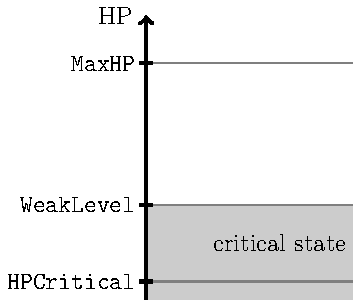
\includegraphics[width=0.3\linewidth]{002_simulation_structure/images/health_global.pdf}
    \caption{The health of the agents is represented by a HP value between \lstinline$HPCritical$ and \lstinline$MaxHP$. All HP values which are below \lstinline$WeakLevel$ are classed as critical. The diagram is not drawn to scale.}
    \label{fig:health_system}
\end{figure}

\subsection{Food and Health: \texorpdfstring{\texttt{updateHP}}{updateHP}}\label{updateHP}
To increase their HP, agents need to eat. However, the amount an agent's HP improves can saturate in a single day; eating more than a certain amount will provide an agent with no extra benefit to their HP. Moreover, eating more food will lead to diminishing returns in terms of HP change. Mathematically, the ideas of diminishing returns and saturation are well captured by the step response of a 1st-order system \eqref{updateHP_general}:

\begin{equation}\label{updateHP_general}
   \texttt{newHP}= \texttt{currentHP} +\underbrace{w(1-e^{\frac{-\texttt{foodTaken}}{\tau}})}_{\texttt{HPChange}}
\end{equation}

The two parameters $w$ and $\tau$ are defined at the beginning of the simulation. The shape of this curve is given in \Cref{fig:updateHP} together with some important parameters.

\begin{figure}[htb]%
    \centering
    \subfloat[\centering Overview]{{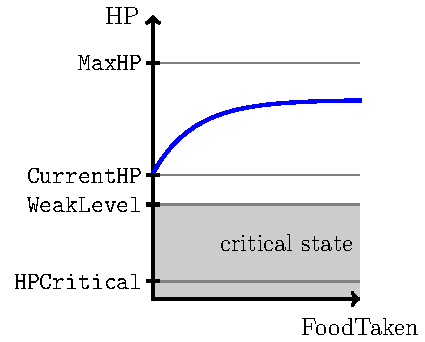
\includegraphics[width=0.36\linewidth]{002_simulation_structure/images/health_updateHP_overview.pdf}}}%
    \qquad
    \subfloat[\centering Detailed representation]{{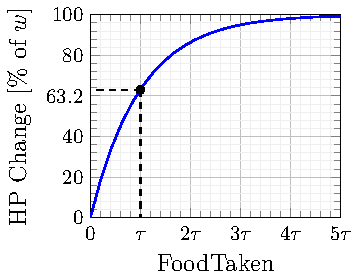
\includegraphics[width=0.36\linewidth]{002_simulation_structure/images/health_updateHP_detailed.pdf}}}%
    \caption{\texttt{updateHP} as a function of the amount of food eaten (``FoodTaken'').}%
    \label{fig:updateHP}%
\end{figure}

It is not possible to gain more HP than $w$ over the duration of one day; this is an intentional limit to prevent an agent's health from improving too quickly. As an example, we can think of an agent that starts from the weak level and wants to reach the maximum HP value. It would take several days for this agent to ``recover'' from this weak level and stabilise its health to a high HP value. 

Note that it is possible for an agent to achieve an HP value that is larger than \texttt{MaxHP} inside \lstinline$hpDecay$. At the end of each day, the \lstinline$hpDecay$ function will apply the cost of living and then bound the final HP value by \lstinline$MaxHP$.


Agents in the critical state are treated differently. For these agents, HP is updated according to equation \eqref{updateHP_critical}:

\begin{equation}\label{updateHP_critical}
    \texttt{newHP} = \min\left\{\texttt{HPCritical}+\texttt{HPReqCToW}, \texttt{currentHP} +w(1-e^{\frac{-\texttt{foodTaken}}{\tau}})\right\}
\end{equation}

\subsection{Cost of Living: \texorpdfstring{\texttt{hpDecay}}{hpDecay}}\label{hpDecay}
At the end of each day, the HP value of the agents will be reduced by the cost of living. The cost of living is larger for an agent with larger HP value than for an agent with lower HP value. This fact is motivated by a simple observation: humans that have stronger bodies and immune systems also need more food to sustain their level of health. The exact relation between HP value, cost of living, and HP value after applying the cost of living is given by the linear relation \eqref{hpDecay_equation}:

\begin{equation}\label{hpDecay_equation}
    \texttt{newHP} = \texttt{currentHP}-\left[b + s(\texttt{currentHP}-\texttt{WeakLevel})\right]
\end{equation}


The parameter $b$ is a (constant) base cost, and $s$ is the slope of the linear function. These parameters are initialised at the beginning of the simulation.

To ensure that the HP value at the end of the day is bounded by \texttt{MaxHP}, we slightly modify (\ref{hpDecay_equation}) to produce (\ref{hpDecay_bounded}):

\begin{equation}\label{hpDecay_bounded}
    \texttt{newHP} =\max\left\{\texttt{MaxHP}, \texttt{currentHP}-\left[b + s(\texttt{currentHP}-\texttt{WeakLevel})\right]\right\}
\end{equation}

For agents in the critical state that gain \texttt{HPReqCToW} HP in a single day, i.e. their HP after eating is

\begin{equation}\label{HPReqCToW}
    \texttt{currentHP} \geq \texttt{HPCritical}+\texttt{HPReqCToW},
\end{equation}

their HP will be set to \texttt{WeakLevel}. Agents in the critical state which do not manage to improve their HP by \lstinline$HPReqCToW$ will be kept in the critical state:

\begin{equation}\label{hpDecay_critical_stay}
    \texttt{newHP} = \texttt{HPCritical}
\end{equation}

with the \texttt{daysAtCritical} counter incremented by 1. If \texttt{daysAtCritical} reaches \texttt{MaxDayCritical}, the agent dies and is replaced. This counter is reset to 0 if an agent exits the critical state.




%%%%%%%%
%%%%%%%% Global Utility
%%%%%%%%
\section{Utility and Social Welfare}\label{utility}

To assess the performance of the agents in the tower as a group, we first need to define a metric. A common choice is the so-called \emph{social welfare}, based on each agent individual utility. For this project, we implement the notion of utility as introduced in \cite{somasPitt}.

Our system is composed of $N$ agents that can perform specific actions in relation with the common pool resources. In a general context, each agent 
$i\in\{1, \ldots, N\}$ takes the following actions at each iteration $t\in\{1,\ldots,\infty\}$:

\begin{enumerate}
    \item Determines the resources it has available, $g_i \in [0,1]$.
    \item Determines its need for resources, $q_i \in [0,1]$.
    \item Makes a provision of resources, $p_i \in [0,1]$.
    \item Makes a demand for resources, $d_i \in [0,1]$.
    \item Receives an allocation of resources, $r_i \in [0,1]$.
    \item Makes an appropriation of resources, $r'_i \in [0,1]$.
\end{enumerate}

In the current setup, the available resources $q_i$ corresponds to the current amount of food on the platform.  The need for resources $q_i$ is defined in relation with the health of the agents. We set the following values to $q_i$:

\begin{equation}\label{resources_needed}
    q_i=\begin{cases}
     \frac{\texttt{numberDaysInCriticalState}}{\texttt{maxDaysInCriticalState}} & \mbox{if } \texttt{currentHP}\leq \texttt{weakLevel}  \\ 
     0 & \mbox{else.}
     \end{cases}
\end{equation}

This way, we ensure that $q_i$ is bounded by 1 and is proportional to the days spent in the critical health zone below \texttt{weakLevel}.

Moreover, the agents do not make any provision $p_i$ to the common pool, as they cannot give food to the platform ($p_i=0$). Their demands for resources is the food they ask for when the platform is at their level. In addition, the agents appropriate all resources they are allocated, so that $r'_i=r_i$.\footnote{We ensure that all these parameters are constrained to the range $[0,1]$ by dividing the mentioned quantities by their maximum values.}

The total resources accrued at the end of an iteration, $R_i$, is hence defined as:

\begin{equation}\label{resources_accrued}
    R_i=r'_i+ (g_i-p_i)
\end{equation}

where each agent will `generate' resources equal to: its appropriation, plus the amount available on the platform, minus the provision made back to the common pool.

Using the above parameters, it is possible to compute the following utility per agent:

\begin{equation}\label{utility_per_agent}
    u_i=\begin{cases}
     \alpha_iq_i + \beta_i(R_i-q_i) & \mbox{if } R_i\geq q_i  \\ 
     \alpha_i R_i - \gamma_i(q_i-R_i) & \mbox{else}
     \end{cases}
\end{equation}


where $\alpha_i$, $\beta_i$ and $\gamma_i$ are tuning parameters that follow the rule $\alpha_i>\gamma_i>\beta_i$. In our work, we use the values $\alpha_i=\alpha=0.2$, $\beta_i=\beta=0.1$, and $\gamma_i=\gamma=0.18$.

Finally, we use \eqref{utility_per_agent} to compute an average global utility, which corresponds to the social welfare \textit{SW} divided by the number of agents:

\begin{equation}\label{utility_eq}
    \mathit{U}=\frac{\sum_i^N u_i}{N}=\frac{\mathit{SW}}{N}
\end{equation}

\section{Technology Stack}

Our technology stack was chosen in the initial meetings of the project, where the individuals were able to propose languages for the frontend and backend, with the backend language used to implement infrastructure and agents. The proposed languages for the backend were:
\begin{enumerate}
    \item Python: A widely used, general purpose programming language with an emphasis on code readability. The language was familiar to a large percentage of the class as a result of having used it in previous projects. 
    \item Go: A less well known language, Go was attractive to the class due to its easy-to-learn nature and easy implementation of concurrency which would be useful in running multiple agents. However, it was unfamiliar to the majority of the class.
    \item C++: A general purpose OOP language, C++ was familiar to a portion of the cohort having studied it in their first year. However, it is not as easy to learn as Go or Python, so this was considered a disadvantage.
\end{enumerate}

After an in-depth review, a vote was cast and Go was the clear preference. Overall, Go was chosen due to its advantages in implementing concurrency and its easy-to-learn nature. In addition to this, the packages in Go would make the code more scalable and readable.

React and Typescript were chosen as the frontend language. They were chosen primarily by the infrastructure team, as this decision would not affect those teams working on agent development. 

%%%%%%%%
%%%%%%%% Simulation Flow
%%%%%%%%
% \section{Simulation Flow}\label{simulation_flow}
% The order in which events happen
% Need a nice diagram for this


% %%%%%%%%
% %%%%%%%% Message Passing
% %%%%%%%%
% \section{Message Passing}\label{message_passing}
% Need a nice diagram for this